% Created by tikzDevice version 0.12.5 on 2024-01-20 16:07:19
% !TEX encoding = UTF-8 Unicode
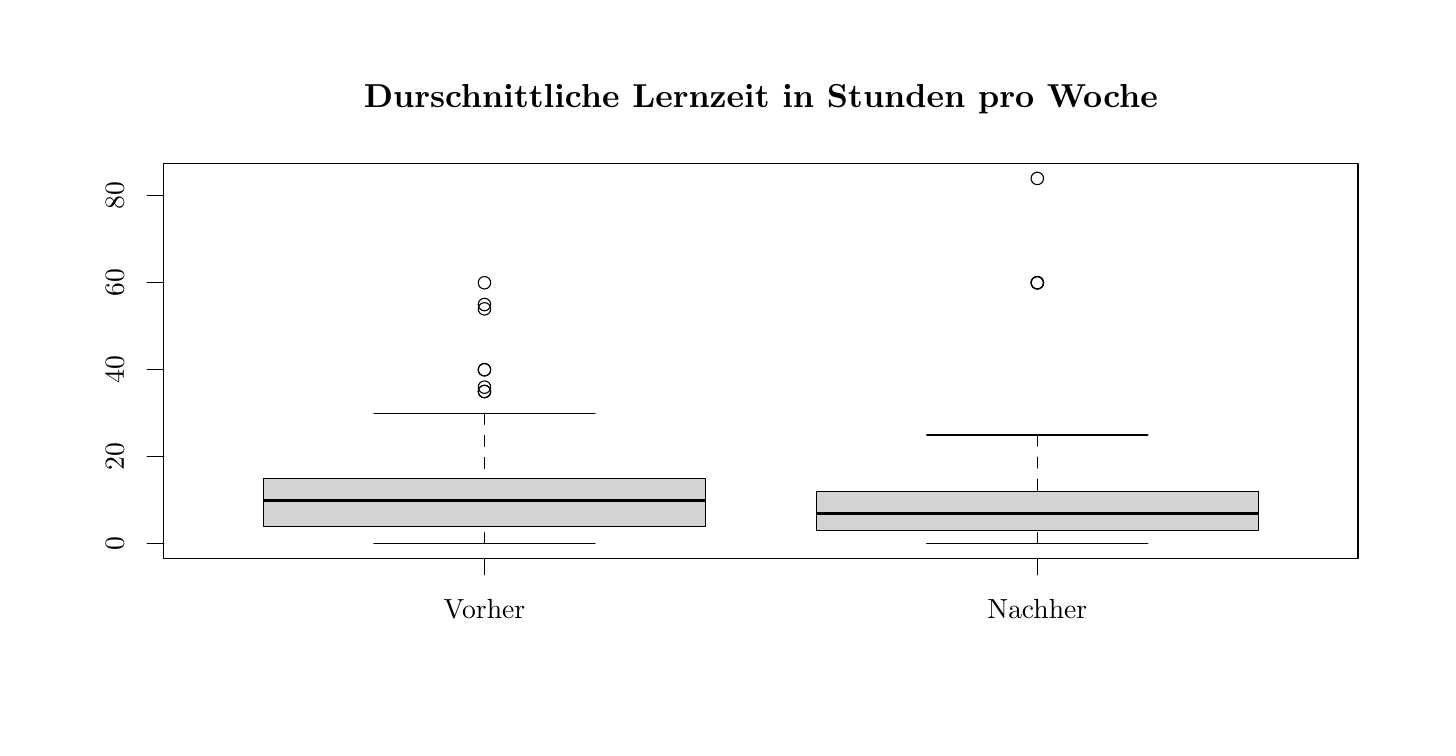
\begin{tikzpicture}[x=1pt,y=1pt]
\definecolor{fillColor}{RGB}{255,255,255}
\path[use as bounding box,fill=fillColor,fill opacity=0.00] (0,0) rectangle (505.89,252.94);
\begin{scope}
\path[clip] ( 49.20, 61.20) rectangle (480.69,203.75);
\definecolor{fillColor}{RGB}{211,211,211}

\path[fill=fillColor] ( 85.16, 72.76) --
	(244.97, 72.76) --
	(244.97, 90.05) --
	( 85.16, 90.05) --
	cycle;
\definecolor{drawColor}{RGB}{0,0,0}

\path[draw=drawColor,line width= 1.2pt,line join=round] ( 85.16, 82.19) -- (244.97, 82.19);

\path[draw=drawColor,line width= 0.4pt,dash pattern=on 4pt off 4pt ,line join=round,line cap=round] (165.06, 66.48) -- (165.06, 72.76);

\path[draw=drawColor,line width= 0.4pt,dash pattern=on 4pt off 4pt ,line join=round,line cap=round] (165.06,113.62) -- (165.06, 90.05);

\path[draw=drawColor,line width= 0.4pt,line join=round,line cap=round] (125.11, 66.48) -- (205.02, 66.48);

\path[draw=drawColor,line width= 0.4pt,line join=round,line cap=round] (125.11,113.62) -- (205.02,113.62);

\path[draw=drawColor,line width= 0.4pt,line join=round,line cap=round] ( 85.16, 72.76) --
	(244.97, 72.76) --
	(244.97, 90.05) --
	( 85.16, 90.05) --
	cycle;

\path[draw=drawColor,line width= 0.4pt,line join=round,line cap=round] (165.06,152.90) circle (  2.25);

\path[draw=drawColor,line width= 0.4pt,line join=round,line cap=round] (165.06,121.47) circle (  2.25);

\path[draw=drawColor,line width= 0.4pt,line join=round,line cap=round] (165.06,129.33) circle (  2.25);

\path[draw=drawColor,line width= 0.4pt,line join=round,line cap=round] (165.06,121.47) circle (  2.25);

\path[draw=drawColor,line width= 0.4pt,line join=round,line cap=round] (165.06,123.04) circle (  2.25);

\path[draw=drawColor,line width= 0.4pt,line join=round,line cap=round] (165.06,160.76) circle (  2.25);

\path[draw=drawColor,line width= 0.4pt,line join=round,line cap=round] (165.06,151.33) circle (  2.25);

\path[draw=drawColor,line width= 0.4pt,line join=round,line cap=round] (165.06,129.33) circle (  2.25);

\path[fill=fillColor] (284.92, 71.19) --
	(444.73, 71.19) --
	(444.73, 85.33) --
	(284.92, 85.33) --
	cycle;

\path[draw=drawColor,line width= 1.2pt,line join=round] (284.92, 77.48) -- (444.73, 77.48);

\path[draw=drawColor,line width= 0.4pt,dash pattern=on 4pt off 4pt ,line join=round,line cap=round] (364.83, 66.48) -- (364.83, 71.19);

\path[draw=drawColor,line width= 0.4pt,dash pattern=on 4pt off 4pt ,line join=round,line cap=round] (364.83,105.76) -- (364.83, 85.33);

\path[draw=drawColor,line width= 0.4pt,line join=round,line cap=round] (324.87, 66.48) -- (404.78, 66.48);

\path[draw=drawColor,line width= 0.4pt,line join=round,line cap=round] (324.87,105.76) -- (404.78,105.76);

\path[draw=drawColor,line width= 0.4pt,line join=round,line cap=round] (284.92, 71.19) --
	(444.73, 71.19) --
	(444.73, 85.33) --
	(284.92, 85.33) --
	cycle;

\path[draw=drawColor,line width= 0.4pt,line join=round,line cap=round] (364.83,160.76) circle (  2.25);

\path[draw=drawColor,line width= 0.4pt,line join=round,line cap=round] (364.83,160.76) circle (  2.25);

\path[draw=drawColor,line width= 0.4pt,line join=round,line cap=round] (364.83,198.47) circle (  2.25);

\path[draw=drawColor,line width= 0.4pt,line join=round,line cap=round] (364.83,160.76) circle (  2.25);
\end{scope}
\begin{scope}
\path[clip] (  0.00,  0.00) rectangle (505.89,252.94);
\definecolor{drawColor}{RGB}{0,0,0}

\path[draw=drawColor,line width= 0.4pt,line join=round,line cap=round] (165.06, 61.20) -- (364.83, 61.20);

\path[draw=drawColor,line width= 0.4pt,line join=round,line cap=round] (165.06, 61.20) -- (165.06, 55.20);

\path[draw=drawColor,line width= 0.4pt,line join=round,line cap=round] (364.83, 61.20) -- (364.83, 55.20);

\node[text=drawColor,anchor=base,inner sep=0pt, outer sep=0pt, scale=  1.00] at (165.06, 39.60) {Vorher};

\node[text=drawColor,anchor=base,inner sep=0pt, outer sep=0pt, scale=  1.00] at (364.83, 39.60) {Nachher};

\path[draw=drawColor,line width= 0.4pt,line join=round,line cap=round] ( 49.20, 66.48) -- ( 49.20,192.18);

\path[draw=drawColor,line width= 0.4pt,line join=round,line cap=round] ( 49.20, 66.48) -- ( 43.20, 66.48);

\path[draw=drawColor,line width= 0.4pt,line join=round,line cap=round] ( 49.20, 97.90) -- ( 43.20, 97.90);

\path[draw=drawColor,line width= 0.4pt,line join=round,line cap=round] ( 49.20,129.33) -- ( 43.20,129.33);

\path[draw=drawColor,line width= 0.4pt,line join=round,line cap=round] ( 49.20,160.76) -- ( 43.20,160.76);

\path[draw=drawColor,line width= 0.4pt,line join=round,line cap=round] ( 49.20,192.18) -- ( 43.20,192.18);

\node[text=drawColor,rotate= 90.00,anchor=base,inner sep=0pt, outer sep=0pt, scale=  1.00] at ( 34.80, 66.48) {0};

\node[text=drawColor,rotate= 90.00,anchor=base,inner sep=0pt, outer sep=0pt, scale=  1.00] at ( 34.80, 97.90) {20};

\node[text=drawColor,rotate= 90.00,anchor=base,inner sep=0pt, outer sep=0pt, scale=  1.00] at ( 34.80,129.33) {40};

\node[text=drawColor,rotate= 90.00,anchor=base,inner sep=0pt, outer sep=0pt, scale=  1.00] at ( 34.80,160.76) {60};

\node[text=drawColor,rotate= 90.00,anchor=base,inner sep=0pt, outer sep=0pt, scale=  1.00] at ( 34.80,192.18) {80};
\end{scope}
\begin{scope}
\path[clip] (  0.00,  0.00) rectangle (505.89,252.94);
\definecolor{drawColor}{RGB}{0,0,0}

\node[text=drawColor,anchor=base,inner sep=0pt, outer sep=0pt, scale=  1.20] at (264.94,224.20) {\bfseries Durschnittliche Lernzeit in Stunden pro Woche};
\end{scope}
\begin{scope}
\path[clip] (  0.00,  0.00) rectangle (505.89,252.94);
\definecolor{drawColor}{RGB}{0,0,0}

\path[draw=drawColor,line width= 0.4pt,line join=round,line cap=round] ( 49.20, 61.20) --
	(480.69, 61.20) --
	(480.69,203.75) --
	( 49.20,203.75) --
	cycle;
\end{scope}
\end{tikzpicture}
